\section{Deployment view}
\paragraph{}In this section we show how our components are really deployed on hardware devices.
\begin{figure}[H]
	\centering
	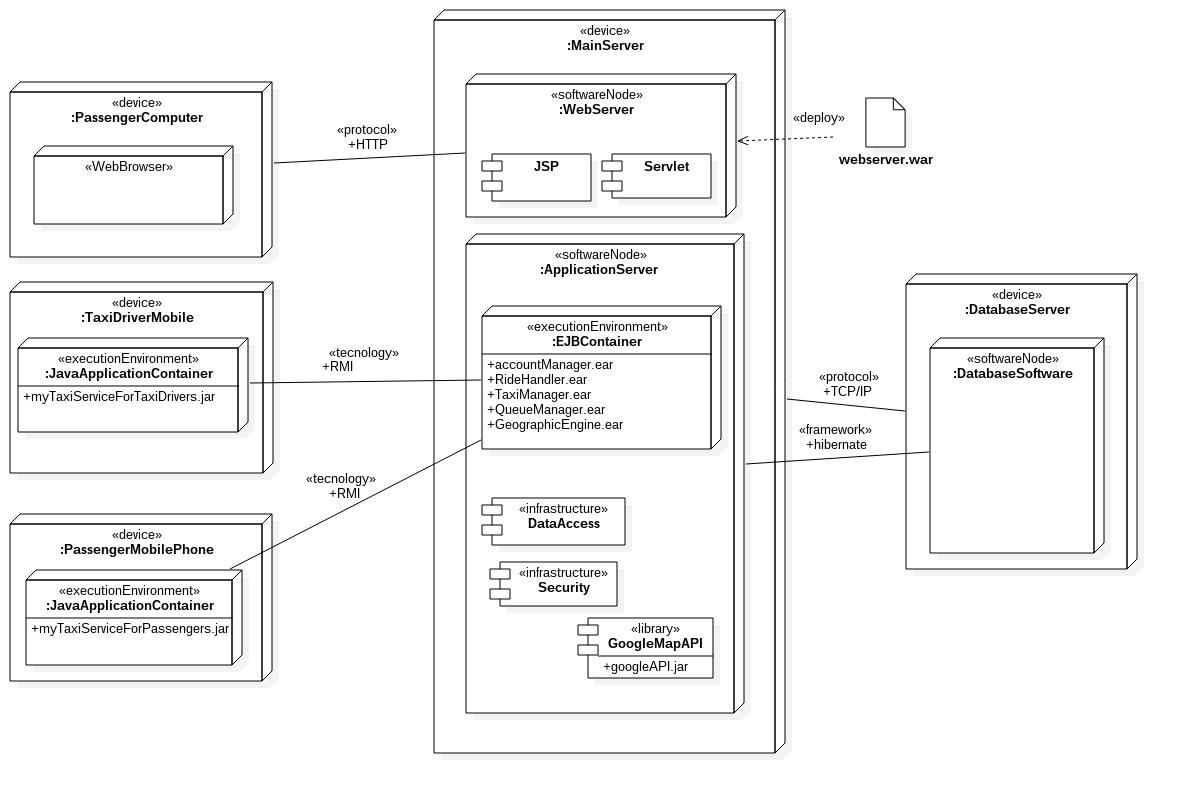
\includegraphics[trim=100 0 0 0,scale=0.40]{../"Analysis Documents"/deploymentView}
\end{figure}
\paragraph{} The UML diagram is self-explicative. We organize our deployed files like this:
\begin{itemize}
	\item On \textit{client side} we show the devices that can interact with our system: a mobile application and a browser for the passenger, and a mobile application for the taxi driver.
	\begin{itemize}
		\item The passenger and taxi driver client applications interact with the system through RMI calls
		\item The browser interact with the Web Server through HTTP protocol
	\end{itemize}
	\item On \textit{server side} both the web server and application server is deployed on the same machine. In particular the Application Server uses the execution environment of the EJB container, with the already specified infrastructural libraries for data access and security. It uses the also the Google Maps API.
	\item The data are stored in an external \textit{database} accessed by the Main Server through the TCP/IP protocol with the support of an Hibernate framework provided by the JEE environment.
\end{itemize}